\documentclass[1p]{elsarticle_modified}
%\bibliographystyle{elsarticle-num}

%\usepackage[colorlinks]{hyperref}
%\usepackage{abbrmath_seonhwa} %\Abb, \Ascr, \Acal ,\Abf, \Afrak
\usepackage{amsfonts}
\usepackage{amssymb}
\usepackage{amsmath}
\usepackage{amsthm}
\usepackage{scalefnt}
\usepackage{amsbsy}
\usepackage{kotex}
\usepackage{caption}
\usepackage{subfig}
\usepackage{color}
\usepackage{graphicx}
\usepackage{xcolor} %% white, black, red, green, blue, cyan, magenta, yellow
\usepackage{float}
\usepackage{setspace}
\usepackage{hyperref}

\usepackage{tikz}
\usetikzlibrary{arrows}

\usepackage{multirow}
\usepackage{array} % fixed length table
\usepackage{hhline}

%%%%%%%%%%%%%%%%%%%%%
\makeatletter
\renewcommand*\env@matrix[1][\arraystretch]{%
	\edef\arraystretch{#1}%
	\hskip -\arraycolsep
	\let\@ifnextchar\new@ifnextchar
	\array{*\c@MaxMatrixCols c}}
\makeatother %https://tex.stackexchange.com/questions/14071/how-can-i-increase-the-line-spacing-in-a-matrix
%%%%%%%%%%%%%%%

\usepackage[normalem]{ulem}

\newcommand{\msout}[1]{\ifmmode\text{\sout{\ensuremath{#1}}}\else\sout{#1}\fi}
%SOURCE: \msout is \stkout macro in https://tex.stackexchange.com/questions/20609/strikeout-in-math-mode

\newcommand{\cancel}[1]{
	\ifmmode
	{\color{red}\msout{#1}}
	\else
	{\color{red}\sout{#1}}
	\fi
}

\newcommand{\add}[1]{
	{\color{blue}\uwave{#1}}
}

\newcommand{\replace}[2]{
	\ifmmode
	{\color{red}\msout{#1}}{\color{blue}\uwave{#2}}
	\else
	{\color{red}\sout{#1}}{\color{blue}\uwave{#2}}
	\fi
}

\newcommand{\Sol}{\mathcal{S}} %segment
\newcommand{\D}{D} %diagram
\newcommand{\A}{\mathcal{A}} %arc


%%%%%%%%%%%%%%%%%%%%%%%%%%%%%5 test

\def\sl{\operatorname{\textup{SL}}(2,\Cbb)}
\def\psl{\operatorname{\textup{PSL}}(2,\Cbb)}
\def\quan{\mkern 1mu \triangleright \mkern 1mu}

\theoremstyle{definition}
\newtheorem{thm}{Theorem}[section]
\newtheorem{prop}[thm]{Proposition}
\newtheorem{lem}[thm]{Lemma}
\newtheorem{ques}[thm]{Question}
\newtheorem{cor}[thm]{Corollary}
\newtheorem{defn}[thm]{Definition}
\newtheorem{exam}[thm]{Example}
\newtheorem{rmk}[thm]{Remark}
\newtheorem{alg}[thm]{Algorithm}

\newcommand{\I}{\sqrt{-1}}
\begin{document}

%\begin{frontmatter}
%
%\title{Boundary parabolic representations of knots up to 8 crossings}
%
%%% Group authors per affiliation:
%\author{Yunhi Cho} 
%\address{Department of Mathematics, University of Seoul, Seoul, Korea}
%\ead{yhcho@uos.ac.kr}
%
%
%\author{Seonhwa Kim} %\fnref{s_kim}}
%\address{Center for Geometry and Physics, Institute for Basic Science, Pohang, 37673, Korea}
%\ead{ryeona17@ibs.re.kr}
%
%\author{Hyuk Kim}
%\address{Department of Mathematical Sciences, Seoul National University, Seoul 08826, Korea}
%\ead{hyukkim@snu.ac.kr}
%
%\author{Seokbeom Yoon}
%\address{Department of Mathematical Sciences, Seoul National University, Seoul, 08826,  Korea}
%\ead{sbyoon15@snu.ac.kr}
%
%\begin{abstract}
%We find all boundary parabolic representation of knots up to 8 crossings.
%
%\end{abstract}
%\begin{keyword}
%    \MSC[2010] 57M25 
%\end{keyword}
%
%\end{frontmatter}

%\linenumbers
%\tableofcontents
%
\newcommand\colored[1]{\textcolor{white}{\rule[-0.35ex]{0.8em}{1.4ex}}\kern-0.8em\color{red} #1}%
%\newcommand\colored[1]{\textcolor{white}{ #1}\kern-2.17ex	\textcolor{white}{ #1}\kern-1.81ex	\textcolor{white}{ #1}\kern-2.15ex\color{red}#1	}

{\Large $\underline{12a_{0150}~(K12a_{0150})}$}

\setlength{\tabcolsep}{10pt}
\renewcommand{\arraystretch}{1.6}
\vspace{1cm}\begin{tabular}{m{100pt}>{\centering\arraybackslash}m{274pt}}
\multirow{5}{120pt}{
	\centering
	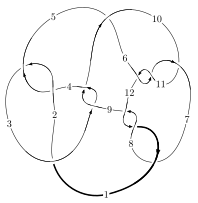
\includegraphics[width=112pt]{../../../GIT/diagram.site/Diagrams/png/951_12a_0150.png}\\
\ \ \ A knot diagram\footnotemark}&
\allowdisplaybreaks
\textbf{Linearized knot diagam} \\
\cline{2-2}
 &
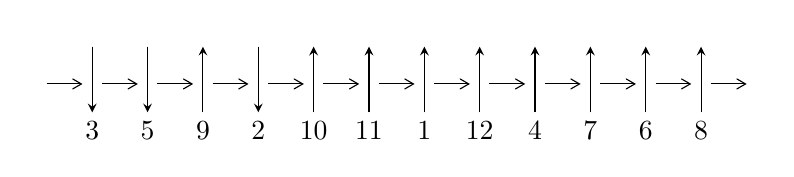
\begin{tikzpicture}[x=20pt, y=17pt]
	% nodes
	\node (C0) at (0, 0) {};
	\node (C1) at (1, 0) {};
	\node (C1U) at (1, +1) {};
	\node (C1D) at (1, -1) {3};

	\node (C2) at (2, 0) {};
	\node (C2U) at (2, +1) {};
	\node (C2D) at (2, -1) {5};

	\node (C3) at (3, 0) {};
	\node (C3U) at (3, +1) {};
	\node (C3D) at (3, -1) {9};

	\node (C4) at (4, 0) {};
	\node (C4U) at (4, +1) {};
	\node (C4D) at (4, -1) {2};

	\node (C5) at (5, 0) {};
	\node (C5U) at (5, +1) {};
	\node (C5D) at (5, -1) {10};

	\node (C6) at (6, 0) {};
	\node (C6U) at (6, +1) {};
	\node (C6D) at (6, -1) {11};

	\node (C7) at (7, 0) {};
	\node (C7U) at (7, +1) {};
	\node (C7D) at (7, -1) {1};

	\node (C8) at (8, 0) {};
	\node (C8U) at (8, +1) {};
	\node (C8D) at (8, -1) {12};

	\node (C9) at (9, 0) {};
	\node (C9U) at (9, +1) {};
	\node (C9D) at (9, -1) {4};

	\node (C10) at (10, 0) {};
	\node (C10U) at (10, +1) {};
	\node (C10D) at (10, -1) {7};

	\node (C11) at (11, 0) {};
	\node (C11U) at (11, +1) {};
	\node (C11D) at (11, -1) {6};

	\node (C12) at (12, 0) {};
	\node (C12U) at (12, +1) {};
	\node (C12D) at (12, -1) {8};
	\node (C13) at (13, 0) {};

	% arrows
	\draw[->,>={angle 60}]
	(C0) edge (C1) (C1) edge (C2) (C2) edge (C3) (C3) edge (C4) (C4) edge (C5) (C5) edge (C6) (C6) edge (C7) (C7) edge (C8) (C8) edge (C9) (C9) edge (C10) (C10) edge (C11) (C11) edge (C12) (C12) edge (C13) ;	\draw[->,>=stealth]
	(C1U) edge (C1D) (C2U) edge (C2D) (C3D) edge (C3U) (C4U) edge (C4D) (C5D) edge (C5U) (C6D) edge (C6U) (C7D) edge (C7U) (C8D) edge (C8U) (C9D) edge (C9U) (C10D) edge (C10U) (C11D) edge (C11U) (C12D) edge (C12U) ;
	\end{tikzpicture} \\
\hhline{~~} \\& 
\textbf{Solving Sequence} \\ \cline{2-2} 
 &
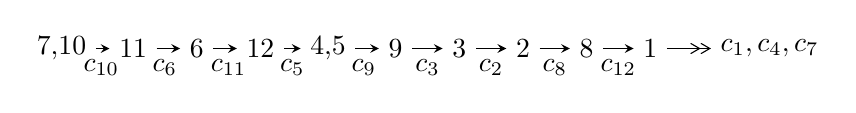
\begin{tikzpicture}[x=23pt, y=7pt]
	% node
	\node (A0) at (-1/8, 0) {7,10};
	\node (A1) at (1, 0) {11};
	\node (A2) at (2, 0) {6};
	\node (A3) at (3, 0) {12};
	\node (A4) at (65/16, 0) {4,5};
	\node (A5) at (41/8, 0) {9};
	\node (A6) at (49/8, 0) {3};
	\node (A7) at (57/8, 0) {2};
	\node (A8) at (65/8, 0) {8};
	\node (A9) at (73/8, 0) {1};
	\node (C1) at (1/2, -1) {$c_{10}$};
	\node (C2) at (3/2, -1) {$c_{6}$};
	\node (C3) at (5/2, -1) {$c_{11}$};
	\node (C4) at (7/2, -1) {$c_{5}$};
	\node (C5) at (37/8, -1) {$c_{9}$};
	\node (C6) at (45/8, -1) {$c_{3}$};
	\node (C7) at (53/8, -1) {$c_{2}$};
	\node (C8) at (61/8, -1) {$c_{8}$};
	\node (C9) at (69/8, -1) {$c_{12}$};
	\node (A10) at (11, 0) {$c_{1},c_{4},c_{7}$};

	% edge
	\draw[->,>=stealth]	
	(A0) edge (A1) (A1) edge (A2) (A2) edge (A3) (A3) edge (A4) (A4) edge (A5) (A5) edge (A6) (A6) edge (A7) (A7) edge (A8) (A8) edge (A9) ;
	\draw[->>,>={angle 60}]	
	(A9) edge (A10);
\end{tikzpicture} \\ 

\end{tabular} \\

\footnotetext{
The image of knot diagram is generated by the software ``\textbf{Draw programme}" developed by Andrew Bartholomew(\url{http://www.layer8.co.uk/maths/draw/index.htm\#Running-draw}), where we modified some parts for our purpose(\url{https://github.com/CATsTAILs/LinksPainter}).
}\phantom \\ \newline 
\centering \textbf{Ideals for irreducible components\footnotemark of $X_{\text{par}}$} 
 
\begin{align*}
I^u_{1}&=\langle 
- u^{35}+13 u^{34}+\cdots+16 b-7,\;-17 u^{35}-37 u^{34}+\cdots+64 a+19,\;u^{36}+19 u^{34}+\cdots-5 u^2-1\rangle \\
I^u_{2}&=\langle 
6.38800\times10^{30} u^{55}-1.52613\times10^{31} u^{54}+\cdots+5.64156\times10^{30} b-1.61757\times10^{32},\\
\phantom{I^u_{2}}&\phantom{= \langle  }-2.85017\times10^{32} u^{55}+2.45748\times10^{32} u^{54}+\cdots+9.59066\times10^{31} a+2.82390\times10^{33},\\
\phantom{I^u_{2}}&\phantom{= \langle  }u^{56}-2 u^{55}+\cdots-56 u+17\rangle \\
I^u_{3}&=\langle 
b,\;- u^2+2 a- u-3,\;u^3+2 u-1\rangle \\
I^u_{4}&=\langle 
a^2+2 a u+2 b+2 a+2 u,\;a^3+2 a^2 u+2 a^2+2 a u+2 u-2,\;u^2+1\rangle \\
I^u_{5}&=\langle 
b,\;u^3+a+u+1,\;u^4+u^3+2 u^2+2 u+1\rangle \\
\\
\end{align*}
\raggedright * 5 irreducible components of $\dim_{\mathbb{C}}=0$, with total 105 representations.\\
\footnotetext{All coefficients of polynomials are rational numbers. But the coefficients are sometimes approximated in decimal forms when there is not enough margin.}
\newpage
\renewcommand{\arraystretch}{1}
\centering \section*{I. $I^u_{1}= \langle - u^{35}+13 u^{34}+\cdots+16 b-7,\;-17 u^{35}-37 u^{34}+\cdots+64 a+19,\;u^{36}+19 u^{34}+\cdots-5 u^2-1 \rangle$}
\flushleft \textbf{(i) Arc colorings}\\
\begin{tabular}{m{7pt} m{180pt} m{7pt} m{180pt} }
\flushright $a_{7}=$&$\begin{pmatrix}0\\u\end{pmatrix}$ \\
\flushright $a_{10}=$&$\begin{pmatrix}1\\0\end{pmatrix}$ \\
\flushright $a_{11}=$&$\begin{pmatrix}1\\- u^2\end{pmatrix}$ \\
\flushright $a_{6}=$&$\begin{pmatrix}- u\\u^3+u\end{pmatrix}$ \\
\flushright $a_{12}=$&$\begin{pmatrix}u^2+1\\- u^4-2 u^2\end{pmatrix}$ \\
\flushright $a_{4}=$&$\begin{pmatrix}0.265625 u^{35}+0.578125 u^{34}+\cdots-5.60938 u-0.296875\\0.0625000 u^{35}-0.812500 u^{34}+\cdots-0.937500 u+0.437500\end{pmatrix}$ \\
\flushright $a_{5}=$&$\begin{pmatrix}- u^3-2 u\\u^3+u\end{pmatrix}$ \\
\flushright $a_{9}=$&$\begin{pmatrix}u^3+2 u\\-\frac{1}{8} u^{34}-\frac{9}{4} u^{32}+\cdots+u+\frac{1}{8}\end{pmatrix}$ \\
\flushright $a_{3}=$&$\begin{pmatrix}0.453125 u^{35}-0.109375 u^{34}+\cdots-5.67188 u+0.0156250\\0.187500 u^{35}+0.812500 u^{34}+\cdots-0.812500 u-0.687500\end{pmatrix}$ \\
\flushright $a_{2}=$&$\begin{pmatrix}0.234375 u^{35}-0.328125 u^{34}+\cdots-4.64063 u-0.453125\\\frac{1}{4} u^{35}+\frac{3}{8} u^{34}+\cdots-\frac{5}{4} u-\frac{1}{8}\end{pmatrix}$ \\
\flushright $a_{8}=$&$\begin{pmatrix}u\\-\frac{1}{8} u^{34}-\frac{9}{4} u^{32}+\cdots+u+\frac{1}{8}\end{pmatrix}$ \\
\flushright $a_{1}=$&$\begin{pmatrix}1\\\frac{1}{8} u^{35}+\frac{9}{4} u^{33}+\cdots-3 u^2-\frac{1}{8} u\end{pmatrix}$\\&\end{tabular}
\flushleft \textbf{(ii) Obstruction class $= -1$}\\~\\
\flushleft \textbf{(iii) Cusp Shapes $= \frac{187}{128} u^{35}+\frac{159}{128} u^{34}+\cdots+\frac{2051}{128} u+\frac{391}{128}$}\\~\\
\newpage\renewcommand{\arraystretch}{1}
\flushleft \textbf{(iv) u-Polynomials at the component}\newline \\
\begin{tabular}{m{50pt}|m{274pt}}
Crossings & \hspace{64pt}u-Polynomials at each crossing \\
\hline $$\begin{aligned}c_{1}\end{aligned}$$&$\begin{aligned}
&u^{36}+16 u^{35}+\cdots+1009 u+16
\end{aligned}$\\
\hline $$\begin{aligned}c_{2},c_{4}\end{aligned}$$&$\begin{aligned}
&u^{36}-4 u^{35}+\cdots+41 u-4
\end{aligned}$\\
\hline $$\begin{aligned}c_{3},c_{9}\end{aligned}$$&$\begin{aligned}
&u^{36}-3 u^{35}+\cdots-200 u+32
\end{aligned}$\\
\hline $$\begin{aligned}c_{5}\end{aligned}$$&$\begin{aligned}
&u^{36}+6 u^{35}+\cdots-1024 u-256
\end{aligned}$\\
\hline $$\begin{aligned}c_{6},c_{7},c_{8}\\c_{10},c_{11},c_{12}\end{aligned}$$&$\begin{aligned}
&u^{36}+19 u^{34}+\cdots-5 u^2-1
\end{aligned}$\\
\hline
\end{tabular}\\~\\
\newpage\renewcommand{\arraystretch}{1}
\flushleft \textbf{(v) Riley Polynomials at the component}\newline \\
\begin{tabular}{m{50pt}|m{274pt}}
Crossings & \hspace{64pt}Riley Polynomials at each crossing \\
\hline $$\begin{aligned}c_{1}\end{aligned}$$&$\begin{aligned}
&y^{36}+12 y^{35}+\cdots-838433 y+256
\end{aligned}$\\
\hline $$\begin{aligned}c_{2},c_{4}\end{aligned}$$&$\begin{aligned}
&y^{36}-16 y^{35}+\cdots-1009 y+16
\end{aligned}$\\
\hline $$\begin{aligned}c_{3},c_{9}\end{aligned}$$&$\begin{aligned}
&y^{36}-21 y^{35}+\cdots-13632 y+1024
\end{aligned}$\\
\hline $$\begin{aligned}c_{5}\end{aligned}$$&$\begin{aligned}
&y^{36}-10 y^{35}+\cdots+1277952 y+65536
\end{aligned}$\\
\hline $$\begin{aligned}c_{6},c_{7},c_{8}\\c_{10},c_{11},c_{12}\end{aligned}$$&$\begin{aligned}
&y^{36}+38 y^{35}+\cdots+10 y+1
\end{aligned}$\\
\hline
\end{tabular}\\~\\
\newpage\flushleft \textbf{(vi) Complex Volumes and Cusp Shapes}
$$\begin{array}{c|c|c}  
\text{Solutions to }I^u_{1}& \I (\text{vol} + \sqrt{-1}CS) & \text{Cusp shape}\\
 \hline 
\begin{aligned}
u &= -0.799527 + 0.176704 I \\
a &= -2.18880 - 0.45142 I \\
b &= \phantom{-}1.268070 - 0.575288 I\end{aligned}
 & \phantom{-}4.74793 - 7.85320 I & \phantom{-}10.04645 + 6.82462 I \\ \hline\begin{aligned}
u &= -0.799527 - 0.176704 I \\
a &= -2.18880 + 0.45142 I \\
b &= \phantom{-}1.268070 + 0.575288 I\end{aligned}
 & \phantom{-}4.74793 + 7.85320 I & \phantom{-}10.04645 - 6.82462 I \\ \hline\begin{aligned}
u &= -0.800607 + 0.101659 I \\
a &= \phantom{-}2.31721 + 0.28975 I \\
b &= -1.291650 + 0.333161 I\end{aligned}
 & \phantom{-}6.52211 - 2.11667 I & \phantom{-}12.90027 + 1.65144 I \\ \hline\begin{aligned}
u &= -0.800607 - 0.101659 I \\
a &= \phantom{-}2.31721 - 0.28975 I \\
b &= -1.291650 - 0.333161 I\end{aligned}
 & \phantom{-}6.52211 + 2.11667 I & \phantom{-}12.90027 - 1.65144 I \\ \hline\begin{aligned}
u &= \phantom{-}0.185932 + 1.257960 I \\
a &= -1.049650 + 0.171429 I \\
b &= \phantom{-}1.49538 - 0.38047 I\end{aligned}
 & -1.32995 - 0.96493 I & \phantom{-}1.34412 - 1.32210 I \\ \hline\begin{aligned}
u &= \phantom{-}0.185932 - 1.257960 I \\
a &= -1.049650 - 0.171429 I \\
b &= \phantom{-}1.49538 + 0.38047 I\end{aligned}
 & -1.32995 + 0.96493 I & \phantom{-}1.34412 + 1.32210 I \\ \hline\begin{aligned}
u &= \phantom{-}0.707581 + 0.074386 I \\
a &= -0.078771 + 0.776564 I \\
b &= \phantom{-}0.233551 - 0.999375 I\end{aligned}
 & \phantom{-}1.47492 + 2.13531 I & \phantom{-}9.68335 - 3.80042 I \\ \hline\begin{aligned}
u &= \phantom{-}0.707581 - 0.074386 I \\
a &= -0.078771 - 0.776564 I \\
b &= \phantom{-}0.233551 + 0.999375 I\end{aligned}
 & \phantom{-}1.47492 - 2.13531 I & \phantom{-}9.68335 + 3.80042 I \\ \hline\begin{aligned}
u &= \phantom{-}0.256428 + 1.268940 I \\
a &= \phantom{-}1.158250 - 0.431595 I \\
b &= -1.50604 + 0.08197 I\end{aligned}
 & -0.50515 + 5.47281 I & \phantom{-}3.56359 - 6.08643 I \\ \hline\begin{aligned}
u &= \phantom{-}0.256428 - 1.268940 I \\
a &= \phantom{-}1.158250 + 0.431595 I \\
b &= -1.50604 - 0.08197 I\end{aligned}
 & -0.50515 - 5.47281 I & \phantom{-}3.56359 + 6.08643 I\\
 \hline 
 \end{array}$$\newpage$$\begin{array}{c|c|c}  
\text{Solutions to }I^u_{1}& \I (\text{vol} + \sqrt{-1}CS) & \text{Cusp shape}\\
 \hline 
\begin{aligned}
u &= -0.655018\phantom{ +0.000000I} \\
a &= -3.09255\phantom{ +0.000000I} \\
b &= \phantom{-}0.837842\phantom{ +0.000000I}\end{aligned}
 & \phantom{-}0.0745611\phantom{ +0.000000I} & \phantom{-}12.4420\phantom{ +0.000000I} \\ \hline\begin{aligned}
u &= -0.270723 + 1.357970 I \\
a &= -0.434177 - 0.095111 I \\
b &= -0.105956 - 1.152130 I\end{aligned}
 & -6.77626 - 4.69556 I & \phantom{-0.000000 } 0 \\ \hline\begin{aligned}
u &= -0.270723 - 1.357970 I \\
a &= -0.434177 + 0.095111 I \\
b &= -0.105956 + 1.152130 I\end{aligned}
 & -6.77626 + 4.69556 I & \phantom{-0.000000 } 0 \\ \hline\begin{aligned}
u &= \phantom{-}0.432384 + 0.427628 I \\
a &= -0.414829 + 0.874160 I \\
b &= \phantom{-}1.078680 - 0.178305 I\end{aligned}
 & \phantom{-}1.50887 - 1.02448 I & \phantom{-}9.47604 - 1.44360 I \\ \hline\begin{aligned}
u &= \phantom{-}0.432384 - 0.427628 I \\
a &= -0.414829 - 0.874160 I \\
b &= \phantom{-}1.078680 + 0.178305 I\end{aligned}
 & \phantom{-}1.50887 + 1.02448 I & \phantom{-}9.47604 + 1.44360 I \\ \hline\begin{aligned}
u &= \phantom{-}0.257005 + 0.526031 I \\
a &= \phantom{-}0.362281 - 0.956728 I \\
b &= -1.160170 - 0.273905 I\end{aligned}
 & \phantom{-}1.25861 + 3.83246 I & \phantom{-}8.43096 - 7.69033 I \\ \hline\begin{aligned}
u &= \phantom{-}0.257005 - 0.526031 I \\
a &= \phantom{-}0.362281 + 0.956728 I \\
b &= -1.160170 + 0.273905 I\end{aligned}
 & \phantom{-}1.25861 - 3.83246 I & \phantom{-}8.43096 + 7.69033 I \\ \hline\begin{aligned}
u &= \phantom{-}0.29960 + 1.38694 I \\
a &= -1.67352 + 0.92125 I \\
b &= \phantom{-}1.085350 + 0.310979 I\end{aligned}
 & -9.07301 + 7.01583 I & \phantom{-0.000000 } 0 \\ \hline\begin{aligned}
u &= \phantom{-}0.29960 - 1.38694 I \\
a &= -1.67352 - 0.92125 I \\
b &= \phantom{-}1.085350 - 0.310979 I\end{aligned}
 & -9.07301 - 7.01583 I & \phantom{-0.000000 } 0 \\ \hline\begin{aligned}
u &= -0.07865 + 1.42029 I \\
a &= -0.398304 - 0.466774 I \\
b &= \phantom{-}0.718949 - 0.847255 I\end{aligned}
 & -9.22257 - 2.95016 I & \phantom{-0.000000 } 0\\
 \hline 
 \end{array}$$\newpage$$\begin{array}{c|c|c}  
\text{Solutions to }I^u_{1}& \I (\text{vol} + \sqrt{-1}CS) & \text{Cusp shape}\\
 \hline 
\begin{aligned}
u &= -0.07865 - 1.42029 I \\
a &= -0.398304 + 0.466774 I \\
b &= \phantom{-}0.718949 + 0.847255 I\end{aligned}
 & -9.22257 + 2.95016 I & \phantom{-0.000000 } 0 \\ \hline\begin{aligned}
u &= -0.32955 + 1.39003 I \\
a &= \phantom{-}0.471381 - 0.002675 I \\
b &= \phantom{-}0.450280 + 1.163260 I\end{aligned}
 & -7.96782 - 9.82231 I & \phantom{-0.000000 } 0 \\ \hline\begin{aligned}
u &= -0.32955 - 1.39003 I \\
a &= \phantom{-}0.471381 + 0.002675 I \\
b &= \phantom{-}0.450280 - 1.163260 I\end{aligned}
 & -7.96782 + 9.82231 I & \phantom{-0.000000 } 0 \\ \hline\begin{aligned}
u &= \phantom{-}0.36777 + 1.38101 I \\
a &= \phantom{-}1.29940 - 1.07583 I \\
b &= -1.31910 - 0.56226 I\end{aligned}
 & -2.87873 + 10.65860 I & \phantom{-0.000000 } 0 \\ \hline\begin{aligned}
u &= \phantom{-}0.36777 - 1.38101 I \\
a &= \phantom{-}1.29940 + 1.07583 I \\
b &= -1.31910 + 0.56226 I\end{aligned}
 & -2.87873 - 10.65860 I & \phantom{-0.000000 } 0 \\ \hline\begin{aligned}
u &= \phantom{-}0.02175 + 1.45011 I \\
a &= \phantom{-}0.585925 + 0.756135 I \\
b &= -0.821813 + 0.809606 I\end{aligned}
 & -12.81680 + 1.42112 I & \phantom{-0.000000 } 0 \\ \hline\begin{aligned}
u &= \phantom{-}0.02175 - 1.45011 I \\
a &= \phantom{-}0.585925 - 0.756135 I \\
b &= -0.821813 - 0.809606 I\end{aligned}
 & -12.81680 - 1.42112 I & \phantom{-0.000000 } 0 \\ \hline\begin{aligned}
u &= \phantom{-}0.38371 + 1.41444 I \\
a &= -1.25562 + 1.21879 I \\
b &= \phantom{-}1.26488 + 0.73094 I\end{aligned}
 & -5.3479 + 16.6018 I & \phantom{-0.000000 } 0 \\ \hline\begin{aligned}
u &= \phantom{-}0.38371 - 1.41444 I \\
a &= -1.25562 - 1.21879 I \\
b &= \phantom{-}1.26488 - 0.73094 I\end{aligned}
 & -5.3479 - 16.6018 I & \phantom{-0.000000 } 0 \\ \hline\begin{aligned}
u &= -0.25014 + 1.49745 I \\
a &= \phantom{-}0.196746 - 0.200364 I \\
b &= \phantom{-}0.623960 + 0.219536 I\end{aligned}
 & -10.76370 - 4.55503 I & \phantom{-0.000000 } 0\\
 \hline 
 \end{array}$$\newpage$$\begin{array}{c|c|c}  
\text{Solutions to }I^u_{1}& \I (\text{vol} + \sqrt{-1}CS) & \text{Cusp shape}\\
 \hline 
\begin{aligned}
u &= -0.25014 - 1.49745 I \\
a &= \phantom{-}0.196746 + 0.200364 I \\
b &= \phantom{-}0.623960 - 0.219536 I\end{aligned}
 & -10.76370 + 4.55503 I & \phantom{-0.000000 } 0 \\ \hline\begin{aligned}
u &= -0.11074 + 1.53043 I \\
a &= \phantom{-}0.086477 + 0.589795 I \\
b &= -0.884099 + 0.624341 I\end{aligned}
 & -12.5319 - 6.8373 I & \phantom{-0.000000 } 0 \\ \hline\begin{aligned}
u &= -0.11074 - 1.53043 I \\
a &= \phantom{-}0.086477 - 0.589795 I \\
b &= -0.884099 - 0.624341 I\end{aligned}
 & -12.5319 + 6.8373 I & \phantom{-0.000000 } 0 \\ \hline\begin{aligned}
u &= \phantom{-}0.361676\phantom{ +0.000000I} \\
a &= -0.636362\phantom{ +0.000000I} \\
b &= \phantom{-}0.360388\phantom{ +0.000000I}\end{aligned}
 & \phantom{-}0.595912\phantom{ +0.000000I} & \phantom{-}16.6720\phantom{ +0.000000I} \\ \hline\begin{aligned}
u &= -0.125553 + 0.232110 I \\
a &= \phantom{-}0.13047 - 2.31300 I \\
b &= -0.229374 - 0.520047 I\end{aligned}
 & -1.60873 - 0.57225 I & -2.19533 + 2.55248 I \\ \hline\begin{aligned}
u &= -0.125553 - 0.232110 I \\
a &= \phantom{-}0.13047 + 2.31300 I \\
b &= -0.229374 + 0.520047 I\end{aligned}
 & -1.60873 + 0.57225 I & -2.19533 - 2.55248 I\\
 \hline 
 \end{array}$$\newpage\newpage\renewcommand{\arraystretch}{1}
\centering \section*{II. $I^u_{2}= \langle 6.39\times10^{30} u^{55}-1.53\times10^{31} u^{54}+\cdots+5.64\times10^{30} b-1.62\times10^{32},\;-2.85\times10^{32} u^{55}+2.46\times10^{32} u^{54}+\cdots+9.59\times10^{31} a+2.82\times10^{33},\;u^{56}-2 u^{55}+\cdots-56 u+17 \rangle$}
\flushleft \textbf{(i) Arc colorings}\\
\begin{tabular}{m{7pt} m{180pt} m{7pt} m{180pt} }
\flushright $a_{7}=$&$\begin{pmatrix}0\\u\end{pmatrix}$ \\
\flushright $a_{10}=$&$\begin{pmatrix}1\\0\end{pmatrix}$ \\
\flushright $a_{11}=$&$\begin{pmatrix}1\\- u^2\end{pmatrix}$ \\
\flushright $a_{6}=$&$\begin{pmatrix}- u\\u^3+u\end{pmatrix}$ \\
\flushright $a_{12}=$&$\begin{pmatrix}u^2+1\\- u^4-2 u^2\end{pmatrix}$ \\
\flushright $a_{4}=$&$\begin{pmatrix}2.97182 u^{55}-2.56237 u^{54}+\cdots+38.6228 u-29.4443\\-1.13231 u^{55}+2.70516 u^{54}+\cdots-67.9361 u+28.6724\end{pmatrix}$ \\
\flushright $a_{5}=$&$\begin{pmatrix}- u^3-2 u\\u^3+u\end{pmatrix}$ \\
\flushright $a_{9}=$&$\begin{pmatrix}1.37378 u^{55}-2.05523 u^{54}+\cdots+22.6847 u-10.9962\\0.0862068 u^{55}+0.310131 u^{54}+\cdots+3.93944 u-6.65451\end{pmatrix}$ \\
\flushright $a_{3}=$&$\begin{pmatrix}0.196643 u^{55}+1.09359 u^{54}+\cdots-62.9416 u+28.7866\\-1.02772 u^{55}+2.29208 u^{54}+\cdots-38.3434 u+7.61269\end{pmatrix}$ \\
\flushright $a_{2}=$&$\begin{pmatrix}-0.813487 u^{55}+2.59847 u^{54}+\cdots-136.206 u+65.7422\\-0.104046 u^{55}+1.60090 u^{54}+\cdots-20.3881 u-5.41843\end{pmatrix}$ \\
\flushright $a_{8}=$&$\begin{pmatrix}-0.275698 u^{55}+0.0983321 u^{54}+\cdots-35.0403 u+22.8321\\1.64947 u^{55}-2.15356 u^{54}+\cdots+59.7250 u-33.8282\end{pmatrix}$ \\
\flushright $a_{1}=$&$\begin{pmatrix}1.53683 u^{55}-2.73915 u^{54}+\cdots+92.2768 u-48.0224\\-0.453063 u^{55}-0.408827 u^{54}+\cdots+7.39298 u+6.68686\end{pmatrix}$\\&\end{tabular}
\flushleft \textbf{(ii) Obstruction class $= -1$}\\~\\
\flushleft \textbf{(iii) Cusp Shapes $= 4.98882 u^{55}-5.95966 u^{54}+\cdots+21.5498 u+4.33068$}\\~\\
\newpage\renewcommand{\arraystretch}{1}
\flushleft \textbf{(iv) u-Polynomials at the component}\newline \\
\begin{tabular}{m{50pt}|m{274pt}}
Crossings & \hspace{64pt}u-Polynomials at each crossing \\
\hline $$\begin{aligned}c_{1}\end{aligned}$$&$\begin{aligned}
&(u^{28}+13 u^{27}+\cdots-7 u+1)^{2}
\end{aligned}$\\
\hline $$\begin{aligned}c_{2},c_{4}\end{aligned}$$&$\begin{aligned}
&(u^{28}-3 u^{27}+\cdots- u+1)^{2}
\end{aligned}$\\
\hline $$\begin{aligned}c_{3},c_{9}\end{aligned}$$&$\begin{aligned}
&(u^{28}+u^{27}+\cdots+8 u+4)^{2}
\end{aligned}$\\
\hline $$\begin{aligned}c_{5}\end{aligned}$$&$\begin{aligned}
&(u^{28}-2 u^{27}+\cdots-22 u+17)^{2}
\end{aligned}$\\
\hline $$\begin{aligned}c_{6},c_{7},c_{8}\\c_{10},c_{11},c_{12}\end{aligned}$$&$\begin{aligned}
&u^{56}-2 u^{55}+\cdots-56 u+17
\end{aligned}$\\
\hline
\end{tabular}\\~\\
\newpage\renewcommand{\arraystretch}{1}
\flushleft \textbf{(v) Riley Polynomials at the component}\newline \\
\begin{tabular}{m{50pt}|m{274pt}}
Crossings & \hspace{64pt}Riley Polynomials at each crossing \\
\hline $$\begin{aligned}c_{1}\end{aligned}$$&$\begin{aligned}
&(y^{28}+7 y^{27}+\cdots-61 y+1)^{2}
\end{aligned}$\\
\hline $$\begin{aligned}c_{2},c_{4}\end{aligned}$$&$\begin{aligned}
&(y^{28}-13 y^{27}+\cdots+7 y+1)^{2}
\end{aligned}$\\
\hline $$\begin{aligned}c_{3},c_{9}\end{aligned}$$&$\begin{aligned}
&(y^{28}-15 y^{27}+\cdots-88 y+16)^{2}
\end{aligned}$\\
\hline $$\begin{aligned}c_{5}\end{aligned}$$&$\begin{aligned}
&(y^{28}-10 y^{27}+\cdots-246 y+289)^{2}
\end{aligned}$\\
\hline $$\begin{aligned}c_{6},c_{7},c_{8}\\c_{10},c_{11},c_{12}\end{aligned}$$&$\begin{aligned}
&y^{56}+42 y^{55}+\cdots-824 y+289
\end{aligned}$\\
\hline
\end{tabular}\\~\\
\newpage\flushleft \textbf{(vi) Complex Volumes and Cusp Shapes}
$$\begin{array}{c|c|c}  
\text{Solutions to }I^u_{2}& \I (\text{vol} + \sqrt{-1}CS) & \text{Cusp shape}\\
 \hline 
\begin{aligned}
u &= -0.699981 + 0.709842 I \\
a &= -0.932475 - 0.375700 I \\
b &= \phantom{-}0.910131 - 0.395689 I\end{aligned}
 & -4.85759 - 4.24816 I & \phantom{-}2.11355 + 6.97904 I \\ \hline\begin{aligned}
u &= -0.699981 - 0.709842 I \\
a &= -0.932475 + 0.375700 I \\
b &= \phantom{-}0.910131 + 0.395689 I\end{aligned}
 & -4.85759 + 4.24816 I & \phantom{-}2.11355 - 6.97904 I \\ \hline\begin{aligned}
u &= -0.405666 + 0.949027 I \\
a &= -1.45587 - 0.57456 I \\
b &= \phantom{-}0.387411 - 0.832689 I\end{aligned}
 & -5.14204 + 1.40144 I & \phantom{-0.000000 } 0. - 1.74630 I \\ \hline\begin{aligned}
u &= -0.405666 - 0.949027 I \\
a &= -1.45587 + 0.57456 I \\
b &= \phantom{-}0.387411 + 0.832689 I\end{aligned}
 & -5.14204 - 1.40144 I & \phantom{-0.000000 -}0. + 1.74630 I \\ \hline\begin{aligned}
u &= \phantom{-}0.910837 + 0.220913 I \\
a &= \phantom{-}2.06125 - 0.14881 I \\
b &= -1.241130 - 0.661367 I\end{aligned}
 & -0.16281 + 11.95450 I & \phantom{-}5.04116 - 8.32221 I \\ \hline\begin{aligned}
u &= \phantom{-}0.910837 - 0.220913 I \\
a &= \phantom{-}2.06125 + 0.14881 I \\
b &= -1.241130 + 0.661367 I\end{aligned}
 & -0.16281 - 11.95450 I & \phantom{-}5.04116 + 8.32221 I \\ \hline\begin{aligned}
u &= -0.779705 + 0.500231 I \\
a &= \phantom{-}0.591475 + 0.474962 I \\
b &= -0.802767 - 0.244916 I\end{aligned}
 & -4.25756 - 0.90628 I & \phantom{-}4.59768 - 1.67094 I \\ \hline\begin{aligned}
u &= -0.779705 - 0.500231 I \\
a &= \phantom{-}0.591475 - 0.474962 I \\
b &= -0.802767 + 0.244916 I\end{aligned}
 & -4.25756 + 0.90628 I & \phantom{-}4.59768 + 1.67094 I \\ \hline\begin{aligned}
u &= -0.352136 + 1.047700 I \\
a &= \phantom{-}0.764728 + 0.330487 I \\
b &= -1.280370 - 0.446560 I\end{aligned}
 & \phantom{-}2.10501 + 3.62399 I & \phantom{-0.000000 } 0 \\ \hline\begin{aligned}
u &= -0.352136 - 1.047700 I \\
a &= \phantom{-}0.764728 - 0.330487 I \\
b &= -1.280370 + 0.446560 I\end{aligned}
 & \phantom{-}2.10501 - 3.62399 I & \phantom{-0.000000 } 0\\
 \hline 
 \end{array}$$\newpage$$\begin{array}{c|c|c}  
\text{Solutions to }I^u_{2}& \I (\text{vol} + \sqrt{-1}CS) & \text{Cusp shape}\\
 \hline 
\begin{aligned}
u &= \phantom{-}0.864130 + 0.172111 I \\
a &= -2.23241 + 0.01733 I \\
b &= \phantom{-}1.262900 + 0.460239 I\end{aligned}
 & \phantom{-}2.03115 + 6.23266 I & \phantom{-}8.14975 - 4.30079 I \\ \hline\begin{aligned}
u &= \phantom{-}0.864130 - 0.172111 I \\
a &= -2.23241 - 0.01733 I \\
b &= \phantom{-}1.262900 - 0.460239 I\end{aligned}
 & \phantom{-}2.03115 - 6.23266 I & \phantom{-}8.14975 + 4.30079 I \\ \hline\begin{aligned}
u &= \phantom{-}0.384208 + 0.766757 I \\
a &= -1.93610 - 0.04267 I \\
b &= \phantom{-}0.611767 - 0.458091 I\end{aligned}
 & -5.69220 + 0.64414 I & -0.353981 + 1.306831 I \\ \hline\begin{aligned}
u &= \phantom{-}0.384208 - 0.766757 I \\
a &= -1.93610 + 0.04267 I \\
b &= \phantom{-}0.611767 + 0.458091 I\end{aligned}
 & -5.69220 - 0.64414 I & -0.353981 - 1.306831 I \\ \hline\begin{aligned}
u &= -0.797014 + 0.216598 I \\
a &= \phantom{-}0.436400 + 0.813553 I \\
b &= -0.387502 - 1.047530 I\end{aligned}
 & -2.87718 - 5.75423 I & \phantom{-}3.89302 + 5.96655 I \\ \hline\begin{aligned}
u &= -0.797014 - 0.216598 I \\
a &= \phantom{-}0.436400 - 0.813553 I \\
b &= -0.387502 + 1.047530 I\end{aligned}
 & -2.87718 + 5.75423 I & \phantom{-}3.89302 - 5.96655 I \\ \hline\begin{aligned}
u &= \phantom{-}0.468961 + 1.091940 I \\
a &= \phantom{-}0.904715 - 0.796492 I \\
b &= -1.147340 + 0.340892 I\end{aligned}
 & -0.76674 - 1.47542 I & \phantom{-0.000000 } 0 \\ \hline\begin{aligned}
u &= \phantom{-}0.468961 - 1.091940 I \\
a &= \phantom{-}0.904715 + 0.796492 I \\
b &= -1.147340 - 0.340892 I\end{aligned}
 & -0.76674 + 1.47542 I & \phantom{-0.000000 } 0 \\ \hline\begin{aligned}
u &= \phantom{-}0.564404 + 1.054850 I \\
a &= -0.731475 + 0.538685 I \\
b &= \phantom{-}1.175470 - 0.589984 I\end{aligned}
 & -2.69009 - 6.77427 I & \phantom{-0.000000 } 0 \\ \hline\begin{aligned}
u &= \phantom{-}0.564404 - 1.054850 I \\
a &= -0.731475 - 0.538685 I \\
b &= \phantom{-}1.175470 + 0.589984 I\end{aligned}
 & -2.69009 + 6.77427 I & \phantom{-0.000000 } 0\\
 \hline 
 \end{array}$$\newpage$$\begin{array}{c|c|c}  
\text{Solutions to }I^u_{2}& \I (\text{vol} + \sqrt{-1}CS) & \text{Cusp shape}\\
 \hline 
\begin{aligned}
u &= -0.358032 + 1.151180 I \\
a &= -0.994941 - 0.598679 I \\
b &= \phantom{-}1.312590 + 0.177484 I\end{aligned}
 & \phantom{-}3.32245 - 2.08114 I & \phantom{-0.000000 } 0 \\ \hline\begin{aligned}
u &= -0.358032 - 1.151180 I \\
a &= -0.994941 + 0.598679 I \\
b &= \phantom{-}1.312590 - 0.177484 I\end{aligned}
 & \phantom{-}3.32245 + 2.08114 I & \phantom{-0.000000 } 0 \\ \hline\begin{aligned}
u &= \phantom{-}0.054476 + 1.226080 I \\
a &= \phantom{-}0.070708 - 0.771010 I \\
b &= -0.376924 - 0.508425 I\end{aligned}
 & -3.06671 + 1.43304 I & \phantom{-0.000000 } 0 \\ \hline\begin{aligned}
u &= \phantom{-}0.054476 - 1.226080 I \\
a &= \phantom{-}0.070708 + 0.771010 I \\
b &= -0.376924 + 0.508425 I\end{aligned}
 & -3.06671 - 1.43304 I & \phantom{-0.000000 } 0 \\ \hline\begin{aligned}
u &= \phantom{-}0.727104 + 0.234303 I \\
a &= \phantom{-}2.86700 - 0.21576 I \\
b &= -0.907099 - 0.252760 I\end{aligned}
 & -3.94179 + 3.28147 I & \phantom{-}5.23266 - 4.99392 I \\ \hline\begin{aligned}
u &= \phantom{-}0.727104 - 0.234303 I \\
a &= \phantom{-}2.86700 + 0.21576 I \\
b &= -0.907099 + 0.252760 I\end{aligned}
 & -3.94179 - 3.28147 I & \phantom{-}5.23266 + 4.99392 I \\ \hline\begin{aligned}
u &= \phantom{-}0.251940 + 1.214590 I \\
a &= \phantom{-}0.623338 - 0.426042 I \\
b &= -0.017123 - 0.961380 I\end{aligned}
 & -1.96777 + 1.34593 I & \phantom{-0.000000 } 0 \\ \hline\begin{aligned}
u &= \phantom{-}0.251940 - 1.214590 I \\
a &= \phantom{-}0.623338 + 0.426042 I \\
b &= -0.017123 + 0.961380 I\end{aligned}
 & -1.96777 - 1.34593 I & \phantom{-0.000000 } 0 \\ \hline\begin{aligned}
u &= \phantom{-}0.065420 + 1.241340 I \\
a &= -1.01865 + 2.07478 I \\
b &= \phantom{-}0.611767 + 0.458091 I\end{aligned}
 & -5.69220 - 0.64414 I & \phantom{-0.000000 } 0 \\ \hline\begin{aligned}
u &= \phantom{-}0.065420 - 1.241340 I \\
a &= -1.01865 - 2.07478 I \\
b &= \phantom{-}0.611767 - 0.458091 I\end{aligned}
 & -5.69220 + 0.64414 I & \phantom{-0.000000 } 0\\
 \hline 
 \end{array}$$\newpage$$\begin{array}{c|c|c}  
\text{Solutions to }I^u_{2}& \I (\text{vol} + \sqrt{-1}CS) & \text{Cusp shape}\\
 \hline 
\begin{aligned}
u &= -0.173270 + 1.242230 I \\
a &= \phantom{-}0.908391 + 1.036680 I \\
b &= \phantom{-}0.387411 + 0.832689 I\end{aligned}
 & -5.14204 - 1.40144 I & \phantom{-0.000000 } 0 \\ \hline\begin{aligned}
u &= -0.173270 - 1.242230 I \\
a &= \phantom{-}0.908391 - 1.036680 I \\
b &= \phantom{-}0.387411 - 0.832689 I\end{aligned}
 & -5.14204 + 1.40144 I & \phantom{-0.000000 } 0 \\ \hline\begin{aligned}
u &= \phantom{-}0.691070 + 0.028094 I \\
a &= -2.45000 + 0.76218 I \\
b &= \phantom{-}1.312590 + 0.177484 I\end{aligned}
 & \phantom{-}3.32245 - 2.08114 I & \phantom{-}9.79595 + 2.78862 I \\ \hline\begin{aligned}
u &= \phantom{-}0.691070 - 0.028094 I \\
a &= -2.45000 - 0.76218 I \\
b &= \phantom{-}1.312590 - 0.177484 I\end{aligned}
 & \phantom{-}3.32245 + 2.08114 I & \phantom{-}9.79595 - 2.78862 I \\ \hline\begin{aligned}
u &= -0.254280 + 1.286460 I \\
a &= \phantom{-}1.76847 + 1.19991 I \\
b &= -0.907099 + 0.252760 I\end{aligned}
 & -3.94179 - 3.28147 I & \phantom{-0.000000 } 0 \\ \hline\begin{aligned}
u &= -0.254280 - 1.286460 I \\
a &= \phantom{-}1.76847 - 1.19991 I \\
b &= -0.907099 - 0.252760 I\end{aligned}
 & -3.94179 + 3.28147 I & \phantom{-0.000000 } 0 \\ \hline\begin{aligned}
u &= \phantom{-}0.286920 + 1.282550 I \\
a &= \phantom{-}0.74733 - 1.53936 I \\
b &= -1.147340 - 0.340892 I\end{aligned}
 & -0.76674 + 1.47542 I & \phantom{-0.000000 } 0 \\ \hline\begin{aligned}
u &= \phantom{-}0.286920 - 1.282550 I \\
a &= \phantom{-}0.74733 + 1.53936 I \\
b &= -1.147340 + 0.340892 I\end{aligned}
 & -0.76674 - 1.47542 I & \phantom{-0.000000 } 0 \\ \hline\begin{aligned}
u &= -0.636644 + 0.157884 I \\
a &= -0.333609 - 1.000990 I \\
b &= -0.017123 + 0.961380 I\end{aligned}
 & -1.96777 - 1.34593 I & \phantom{-}5.91932 + 0.66126 I \\ \hline\begin{aligned}
u &= -0.636644 - 0.157884 I \\
a &= -0.333609 + 1.000990 I \\
b &= -0.017123 - 0.961380 I\end{aligned}
 & -1.96777 + 1.34593 I & \phantom{-}5.91932 - 0.66126 I\\
 \hline 
 \end{array}$$\newpage$$\begin{array}{c|c|c}  
\text{Solutions to }I^u_{2}& \I (\text{vol} + \sqrt{-1}CS) & \text{Cusp shape}\\
 \hline 
\begin{aligned}
u &= \phantom{-}0.291088 + 1.313610 I \\
a &= -0.713814 + 0.243496 I \\
b &= -0.387502 + 1.047530 I\end{aligned}
 & -2.87718 + 5.75423 I & \phantom{-0.000000 } 0 \\ \hline\begin{aligned}
u &= \phantom{-}0.291088 - 1.313610 I \\
a &= -0.713814 - 0.243496 I \\
b &= -0.387502 - 1.047530 I\end{aligned}
 & -2.87718 - 5.75423 I & \phantom{-0.000000 } 0 \\ \hline\begin{aligned}
u &= -0.405124 + 0.480475 I \\
a &= \phantom{-}1.058260 - 0.685910 I \\
b &= -0.376924 + 0.508425 I\end{aligned}
 & -3.06671 - 1.43304 I & \phantom{-}5.58225 + 4.97603 I \\ \hline\begin{aligned}
u &= -0.405124 - 0.480475 I \\
a &= \phantom{-}1.058260 + 0.685910 I \\
b &= -0.376924 - 0.508425 I\end{aligned}
 & -3.06671 + 1.43304 I & \phantom{-}5.58225 - 4.97603 I \\ \hline\begin{aligned}
u &= -0.342351 + 1.329390 I \\
a &= -1.15193 - 1.31181 I \\
b &= \phantom{-}1.262900 - 0.460239 I\end{aligned}
 & \phantom{-}2.03115 - 6.23266 I & \phantom{-0.000000 } 0 \\ \hline\begin{aligned}
u &= -0.342351 - 1.329390 I \\
a &= -1.15193 + 1.31181 I \\
b &= \phantom{-}1.262900 + 0.460239 I\end{aligned}
 & \phantom{-}2.03115 + 6.23266 I & \phantom{-0.000000 } 0 \\ \hline\begin{aligned}
u &= \phantom{-}0.254428 + 1.359510 I \\
a &= -0.57743 + 1.67051 I \\
b &= \phantom{-}1.175470 + 0.589984 I\end{aligned}
 & -2.69009 + 6.77427 I & \phantom{-0.000000 } 0 \\ \hline\begin{aligned}
u &= \phantom{-}0.254428 - 1.359510 I \\
a &= -0.57743 - 1.67051 I \\
b &= \phantom{-}1.175470 - 0.589984 I\end{aligned}
 & -2.69009 - 6.77427 I & \phantom{-0.000000 } 0 \\ \hline\begin{aligned}
u &= \phantom{-}0.591934 + 0.141506 I \\
a &= \phantom{-}2.29632 - 1.21300 I \\
b &= -1.280370 - 0.446560 I\end{aligned}
 & \phantom{-}2.10501 + 3.62399 I & \phantom{-}8.20871 - 2.76186 I \\ \hline\begin{aligned}
u &= \phantom{-}0.591934 - 0.141506 I \\
a &= \phantom{-}2.29632 + 1.21300 I \\
b &= -1.280370 + 0.446560 I\end{aligned}
 & \phantom{-}2.10501 - 3.62399 I & \phantom{-}8.20871 + 2.76186 I\\
 \hline 
 \end{array}$$\newpage$$\begin{array}{c|c|c}  
\text{Solutions to }I^u_{2}& \I (\text{vol} + \sqrt{-1}CS) & \text{Cusp shape}\\
 \hline 
\begin{aligned}
u &= -0.003051 + 1.410480 I \\
a &= \phantom{-}0.649306 + 0.505190 I \\
b &= \phantom{-}0.910131 + 0.395689 I\end{aligned}
 & -4.85759 + 4.24816 I & \phantom{-0.000000 } 0 \\ \hline\begin{aligned}
u &= -0.003051 - 1.410480 I \\
a &= \phantom{-}0.649306 - 0.505190 I \\
b &= \phantom{-}0.910131 - 0.395689 I\end{aligned}
 & -4.85759 - 4.24816 I & \phantom{-0.000000 } 0 \\ \hline\begin{aligned}
u &= \phantom{-}0.136440 + 1.404460 I \\
a &= -0.588564 - 0.154002 I \\
b &= -0.802767 + 0.244916 I\end{aligned}
 & -4.25756 + 0.90628 I & \phantom{-0.000000 } 0 \\ \hline\begin{aligned}
u &= \phantom{-}0.136440 - 1.404460 I \\
a &= -0.588564 + 0.154002 I \\
b &= -0.802767 - 0.244916 I\end{aligned}
 & -4.25756 - 0.90628 I & \phantom{-0.000000 } 0 \\ \hline\begin{aligned}
u &= -0.33611 + 1.37531 I \\
a &= \phantom{-}1.07544 + 1.49026 I \\
b &= -1.241130 + 0.661367 I\end{aligned}
 & -0.16281 - 11.95450 I & \phantom{-0.000000 } 0 \\ \hline\begin{aligned}
u &= -0.33611 - 1.37531 I \\
a &= \phantom{-}1.07544 - 1.49026 I \\
b &= -1.241130 - 0.661367 I\end{aligned}
 & -0.16281 + 11.95450 I & \phantom{-0.000000 } 0\\
 \hline 
 \end{array}$$\newpage\newpage\renewcommand{\arraystretch}{1}
\centering \section*{III. $I^u_{3}= \langle b,\;- u^2+2 a- u-3,\;u^3+2 u-1 \rangle$}
\flushleft \textbf{(i) Arc colorings}\\
\begin{tabular}{m{7pt} m{180pt} m{7pt} m{180pt} }
\flushright $a_{7}=$&$\begin{pmatrix}0\\u\end{pmatrix}$ \\
\flushright $a_{10}=$&$\begin{pmatrix}1\\0\end{pmatrix}$ \\
\flushright $a_{11}=$&$\begin{pmatrix}1\\- u^2\end{pmatrix}$ \\
\flushright $a_{6}=$&$\begin{pmatrix}- u\\- u+1\end{pmatrix}$ \\
\flushright $a_{12}=$&$\begin{pmatrix}u^2+1\\- u\end{pmatrix}$ \\
\flushright $a_{4}=$&$\begin{pmatrix}\frac{1}{2} u^2+\frac{1}{2} u+\frac{3}{2}\\0\end{pmatrix}$ \\
\flushright $a_{5}=$&$\begin{pmatrix}-1\\- u+1\end{pmatrix}$ \\
\flushright $a_{9}=$&$\begin{pmatrix}1\\0\end{pmatrix}$ \\
\flushright $a_{3}=$&$\begin{pmatrix}\frac{1}{2} u^2+\frac{1}{2} u+\frac{3}{2}\\0\end{pmatrix}$ \\
\flushright $a_{2}=$&$\begin{pmatrix}\frac{1}{2} u^2+\frac{1}{2} u+\frac{5}{2}\\u-1\end{pmatrix}$ \\
\flushright $a_{8}=$&$\begin{pmatrix}u\\u^2\end{pmatrix}$ \\
\flushright $a_{1}=$&$\begin{pmatrix}1\\u-1\end{pmatrix}$\\&\end{tabular}
\flushleft \textbf{(ii) Obstruction class $= 1$}\\~\\
\flushleft \textbf{(iii) Cusp Shapes $= \frac{7}{4} u^2+\frac{21}{4} u+\frac{9}{4}$}\\~\\
\newpage\renewcommand{\arraystretch}{1}
\flushleft \textbf{(iv) u-Polynomials at the component}\newline \\
\begin{tabular}{m{50pt}|m{274pt}}
Crossings & \hspace{64pt}u-Polynomials at each crossing \\
\hline $$\begin{aligned}c_{1},c_{2}\end{aligned}$$&$\begin{aligned}
&(u-1)^3
\end{aligned}$\\
\hline $$\begin{aligned}c_{3},c_{9}\end{aligned}$$&$\begin{aligned}
&u^3
\end{aligned}$\\
\hline $$\begin{aligned}c_{4}\end{aligned}$$&$\begin{aligned}
&(u+1)^3
\end{aligned}$\\
\hline $$\begin{aligned}c_{5}\end{aligned}$$&$\begin{aligned}
&u^3+3 u^2+5 u+2
\end{aligned}$\\
\hline $$\begin{aligned}c_{6},c_{7},c_{8}\end{aligned}$$&$\begin{aligned}
&u^3+2 u+1
\end{aligned}$\\
\hline $$\begin{aligned}c_{10},c_{11},c_{12}\end{aligned}$$&$\begin{aligned}
&u^3+2 u-1
\end{aligned}$\\
\hline
\end{tabular}\\~\\
\newpage\renewcommand{\arraystretch}{1}
\flushleft \textbf{(v) Riley Polynomials at the component}\newline \\
\begin{tabular}{m{50pt}|m{274pt}}
Crossings & \hspace{64pt}Riley Polynomials at each crossing \\
\hline $$\begin{aligned}c_{1},c_{2},c_{4}\end{aligned}$$&$\begin{aligned}
&(y-1)^3
\end{aligned}$\\
\hline $$\begin{aligned}c_{3},c_{9}\end{aligned}$$&$\begin{aligned}
&y^3
\end{aligned}$\\
\hline $$\begin{aligned}c_{5}\end{aligned}$$&$\begin{aligned}
&y^3+y^2+13 y-4
\end{aligned}$\\
\hline $$\begin{aligned}c_{6},c_{7},c_{8}\\c_{10},c_{11},c_{12}\end{aligned}$$&$\begin{aligned}
&y^3+4 y^2+4 y-1
\end{aligned}$\\
\hline
\end{tabular}\\~\\
\newpage\flushleft \textbf{(vi) Complex Volumes and Cusp Shapes}
$$\begin{array}{c|c|c}  
\text{Solutions to }I^u_{3}& \I (\text{vol} + \sqrt{-1}CS) & \text{Cusp shape}\\
 \hline 
\begin{aligned}
u &= -0.22670 + 1.46771 I \\
a &= \phantom{-}0.335258 + 0.401127 I \\
b &= \phantom{-0.000000 } 0\end{aligned}
 & -11.08570 - 5.13794 I & -2.62004 + 6.54094 I \\ \hline\begin{aligned}
u &= -0.22670 - 1.46771 I \\
a &= \phantom{-}0.335258 - 0.401127 I \\
b &= \phantom{-0.000000 } 0\end{aligned}
 & -11.08570 + 5.13794 I & -2.62004 - 6.54094 I \\ \hline\begin{aligned}
u &= \phantom{-}0.453398\phantom{ +0.000000I} \\
a &= \phantom{-}1.82948\phantom{ +0.000000I} \\
b &= \phantom{-0.000000 } 0\end{aligned}
 & -0.857735\phantom{ +0.000000I} & \phantom{-}4.99010\phantom{ +0.000000I}\\
 \hline 
 \end{array}$$\newpage\newpage\renewcommand{\arraystretch}{1}
\centering \section*{IV. $I^u_{4}= \langle a^2+2 a u+2 b+2 a+2 u,\;a^3+2 a^2 u+2 a^2+2 a u+2 u-2,\;u^2+1 \rangle$}
\flushleft \textbf{(i) Arc colorings}\\
\begin{tabular}{m{7pt} m{180pt} m{7pt} m{180pt} }
\flushright $a_{7}=$&$\begin{pmatrix}0\\u\end{pmatrix}$ \\
\flushright $a_{10}=$&$\begin{pmatrix}1\\0\end{pmatrix}$ \\
\flushright $a_{11}=$&$\begin{pmatrix}1\\1\end{pmatrix}$ \\
\flushright $a_{6}=$&$\begin{pmatrix}- u\\0\end{pmatrix}$ \\
\flushright $a_{12}=$&$\begin{pmatrix}0\\1\end{pmatrix}$ \\
\flushright $a_{4}=$&$\begin{pmatrix}a\\-\frac{1}{2} a^2- a u- a- u\end{pmatrix}$ \\
\flushright $a_{5}=$&$\begin{pmatrix}- u\\0\end{pmatrix}$ \\
\flushright $a_{9}=$&$\begin{pmatrix}u\\\frac{1}{2} a^2 u+\frac{1}{2} a u-\frac{1}{2} a+1\end{pmatrix}$ \\
\flushright $a_{3}=$&$\begin{pmatrix}\frac{1}{2} a^2 u+a u-1\\\frac{1}{2} a u+\frac{1}{2} a+u\end{pmatrix}$ \\
\flushright $a_{2}=$&$\begin{pmatrix}\frac{1}{2} a^2 u+\frac{1}{2} a u-\frac{1}{2} a- u-1\\\frac{1}{2} a u+\frac{1}{2} a+u\end{pmatrix}$ \\
\flushright $a_{8}=$&$\begin{pmatrix}u\\\frac{1}{2} a^2 u+\frac{1}{2} a u-\frac{1}{2} a+u+1\end{pmatrix}$ \\
\flushright $a_{1}=$&$\begin{pmatrix}-1\\-\frac{1}{2} a^2-\frac{1}{2} a u-\frac{1}{2} a+u\end{pmatrix}$\\&\end{tabular}
\flushleft \textbf{(ii) Obstruction class $= 1$}\\~\\
\flushleft \textbf{(iii) Cusp Shapes $= -2 a u+2 a+4$}\\~\\
\newpage\renewcommand{\arraystretch}{1}
\flushleft \textbf{(iv) u-Polynomials at the component}\newline \\
\begin{tabular}{m{50pt}|m{274pt}}
Crossings & \hspace{64pt}u-Polynomials at each crossing \\
\hline $$\begin{aligned}c_{1}\end{aligned}$$&$\begin{aligned}
&(u^3- u^2+2 u-1)^2
\end{aligned}$\\
\hline $$\begin{aligned}c_{2}\end{aligned}$$&$\begin{aligned}
&(u^3+u^2-1)^2
\end{aligned}$\\
\hline $$\begin{aligned}c_{3},c_{9}\end{aligned}$$&$\begin{aligned}
&u^6-3 u^4+2 u^2+1
\end{aligned}$\\
\hline $$\begin{aligned}c_{4}\end{aligned}$$&$\begin{aligned}
&(u^3- u^2+1)^2
\end{aligned}$\\
\hline $$\begin{aligned}c_{5}\end{aligned}$$&$\begin{aligned}
&u^6
\end{aligned}$\\
\hline $$\begin{aligned}c_{6},c_{7},c_{8}\\c_{10},c_{11},c_{12}\end{aligned}$$&$\begin{aligned}
&(u^2+1)^3
\end{aligned}$\\
\hline
\end{tabular}\\~\\
\newpage\renewcommand{\arraystretch}{1}
\flushleft \textbf{(v) Riley Polynomials at the component}\newline \\
\begin{tabular}{m{50pt}|m{274pt}}
Crossings & \hspace{64pt}Riley Polynomials at each crossing \\
\hline $$\begin{aligned}c_{1}\end{aligned}$$&$\begin{aligned}
&(y^3+3 y^2+2 y-1)^2
\end{aligned}$\\
\hline $$\begin{aligned}c_{2},c_{4}\end{aligned}$$&$\begin{aligned}
&(y^3- y^2+2 y-1)^2
\end{aligned}$\\
\hline $$\begin{aligned}c_{3},c_{9}\end{aligned}$$&$\begin{aligned}
&(y^3-3 y^2+2 y+1)^2
\end{aligned}$\\
\hline $$\begin{aligned}c_{5}\end{aligned}$$&$\begin{aligned}
&y^6
\end{aligned}$\\
\hline $$\begin{aligned}c_{6},c_{7},c_{8}\\c_{10},c_{11},c_{12}\end{aligned}$$&$\begin{aligned}
&(y+1)^6
\end{aligned}$\\
\hline
\end{tabular}\\~\\
\newpage\flushleft \textbf{(vi) Complex Volumes and Cusp Shapes}
$$\begin{array}{c|c|c}  
\text{Solutions to }I^u_{4}& \I (\text{vol} + \sqrt{-1}CS) & \text{Cusp shape}\\
 \hline 
\begin{aligned}
u &= \phantom{-0.000000 -}1.000000 I \\
a &= -0.867423 + 0.622301 I \\
b &= \phantom{-}1.307140 - 0.215080 I\end{aligned}
 & -0.26574 + 2.82812 I & \phantom{-}3.50976 - 2.97945 I \\ \hline\begin{aligned}
u &= \phantom{-0.000000 -}1.000000 I \\
a &= \phantom{-}0.622301 - 0.867423 I \\
b &= -1.307140 - 0.215080 I\end{aligned}
 & -0.26574 - 2.82812 I & \phantom{-}3.50976 + 2.97945 I \\ \hline\begin{aligned}
u &= \phantom{-0.000000 -}1.000000 I \\
a &= -1.75488 - 1.75488 I \\
b &= \phantom{-0.000000 } -0.569840 I\end{aligned}
 & -4.40332\phantom{ +0.000000I} & -3.01951 + 0. I\phantom{ +0.000000I} \\ \hline\begin{aligned}
u &= \phantom{-0.000000 } -1.000000 I \\
a &= -0.867423 - 0.622301 I \\
b &= \phantom{-}1.307140 + 0.215080 I\end{aligned}
 & -0.26574 - 2.82812 I & \phantom{-}3.50976 + 2.97945 I \\ \hline\begin{aligned}
u &= \phantom{-0.000000 } -1.000000 I \\
a &= \phantom{-}0.622301 + 0.867423 I \\
b &= -1.307140 + 0.215080 I\end{aligned}
 & -0.26574 + 2.82812 I & \phantom{-}3.50976 - 2.97945 I \\ \hline\begin{aligned}
u &= \phantom{-0.000000 } -1.000000 I \\
a &= -1.75488 + 1.75488 I \\
b &= \phantom{-0.000000 -}0.569840 I\end{aligned}
 & -4.40332\phantom{ +0.000000I} & -3.01951 + 0. I\phantom{ +0.000000I}\\
 \hline 
 \end{array}$$\newpage\newpage\renewcommand{\arraystretch}{1}
\centering \section*{V. $I^u_{5}= \langle b,\;u^3+a+u+1,\;u^4+u^3+2 u^2+2 u+1 \rangle$}
\flushleft \textbf{(i) Arc colorings}\\
\begin{tabular}{m{7pt} m{180pt} m{7pt} m{180pt} }
\flushright $a_{7}=$&$\begin{pmatrix}0\\u\end{pmatrix}$ \\
\flushright $a_{10}=$&$\begin{pmatrix}1\\0\end{pmatrix}$ \\
\flushright $a_{11}=$&$\begin{pmatrix}1\\- u^2\end{pmatrix}$ \\
\flushright $a_{6}=$&$\begin{pmatrix}- u\\u^3+u\end{pmatrix}$ \\
\flushright $a_{12}=$&$\begin{pmatrix}u^2+1\\u^3+2 u+1\end{pmatrix}$ \\
\flushright $a_{4}=$&$\begin{pmatrix}- u^3- u-1\\0\end{pmatrix}$ \\
\flushright $a_{5}=$&$\begin{pmatrix}- u^3-2 u\\u^3+u\end{pmatrix}$ \\
\flushright $a_{9}=$&$\begin{pmatrix}1\\0\end{pmatrix}$ \\
\flushright $a_{3}=$&$\begin{pmatrix}- u^3- u-1\\0\end{pmatrix}$ \\
\flushright $a_{2}=$&$\begin{pmatrix}u-1\\- u^3- u\end{pmatrix}$ \\
\flushright $a_{8}=$&$\begin{pmatrix}2 u^3+u^2+3 u+3\\- u^3- u^2- u-2\end{pmatrix}$ \\
\flushright $a_{1}=$&$\begin{pmatrix}u^3+2 u\\- u^3- u\end{pmatrix}$\\&\end{tabular}
\flushleft \textbf{(ii) Obstruction class $= 1$}\\~\\
\flushleft \textbf{(iii) Cusp Shapes $= 4 u^3+4 u+3$}\\~\\
\newpage\renewcommand{\arraystretch}{1}
\flushleft \textbf{(iv) u-Polynomials at the component}\newline \\
\begin{tabular}{m{50pt}|m{274pt}}
Crossings & \hspace{64pt}u-Polynomials at each crossing \\
\hline $$\begin{aligned}c_{1},c_{2}\end{aligned}$$&$\begin{aligned}
&(u-1)^4
\end{aligned}$\\
\hline $$\begin{aligned}c_{3},c_{9}\end{aligned}$$&$\begin{aligned}
&u^4
\end{aligned}$\\
\hline $$\begin{aligned}c_{4}\end{aligned}$$&$\begin{aligned}
&(u+1)^4
\end{aligned}$\\
\hline $$\begin{aligned}c_{5}\end{aligned}$$&$\begin{aligned}
&(u^2- u+1)^2
\end{aligned}$\\
\hline $$\begin{aligned}c_{6},c_{7},c_{8}\end{aligned}$$&$\begin{aligned}
&u^4- u^3+2 u^2-2 u+1
\end{aligned}$\\
\hline $$\begin{aligned}c_{10},c_{11},c_{12}\end{aligned}$$&$\begin{aligned}
&u^4+u^3+2 u^2+2 u+1
\end{aligned}$\\
\hline
\end{tabular}\\~\\
\newpage\renewcommand{\arraystretch}{1}
\flushleft \textbf{(v) Riley Polynomials at the component}\newline \\
\begin{tabular}{m{50pt}|m{274pt}}
Crossings & \hspace{64pt}Riley Polynomials at each crossing \\
\hline $$\begin{aligned}c_{1},c_{2},c_{4}\end{aligned}$$&$\begin{aligned}
&(y-1)^4
\end{aligned}$\\
\hline $$\begin{aligned}c_{3},c_{9}\end{aligned}$$&$\begin{aligned}
&y^4
\end{aligned}$\\
\hline $$\begin{aligned}c_{5}\end{aligned}$$&$\begin{aligned}
&(y^2+y+1)^2
\end{aligned}$\\
\hline $$\begin{aligned}c_{6},c_{7},c_{8}\\c_{10},c_{11},c_{12}\end{aligned}$$&$\begin{aligned}
&y^4+3 y^3+2 y^2+1
\end{aligned}$\\
\hline
\end{tabular}\\~\\
\newpage\flushleft \textbf{(vi) Complex Volumes and Cusp Shapes}
$$\begin{array}{c|c|c}  
\text{Solutions to }I^u_{5}& \I (\text{vol} + \sqrt{-1}CS) & \text{Cusp shape}\\
 \hline 
\begin{aligned}
u &= -0.621744 + 0.440597 I \\
a &= -0.500000 - 0.866025 I \\
b &= \phantom{-0.000000 } 0\end{aligned}
 & -4.93480 - 2.02988 I & \phantom{-}1.0000 + 3.46410 I \\ \hline\begin{aligned}
u &= -0.621744 - 0.440597 I \\
a &= -0.500000 + 0.866025 I \\
b &= \phantom{-0.000000 } 0\end{aligned}
 & -4.93480 + 2.02988 I & \phantom{-}1.0000 - 3.46410 I \\ \hline\begin{aligned}
u &= \phantom{-}0.121744 + 1.306620 I \\
a &= -0.500000 + 0.866025 I \\
b &= \phantom{-0.000000 } 0\end{aligned}
 & -4.93480 + 2.02988 I & \phantom{-}1.00000 - 3.46410 I \\ \hline\begin{aligned}
u &= \phantom{-}0.121744 - 1.306620 I \\
a &= -0.500000 - 0.866025 I \\
b &= \phantom{-0.000000 } 0\end{aligned}
 & -4.93480 - 2.02988 I & \phantom{-}1.00000 + 3.46410 I\\
 \hline 
 \end{array}$$\newpage
\newpage\renewcommand{\arraystretch}{1}
\centering \section*{ VI. u-Polynomials}
\begin{tabular}{m{50pt}|m{274pt}}
Crossings & \hspace{64pt}u-Polynomials at each crossing \\
\hline $$\begin{aligned}c_{1}\end{aligned}$$&$\begin{aligned}
&((u-1)^7)(u^3- u^2+2 u-1)^2(u^{28}+13 u^{27}+\cdots-7 u+1)^{2}\\
&\cdot(u^{36}+16 u^{35}+\cdots+1009 u+16)
\end{aligned}$\\
\hline $$\begin{aligned}c_{2}\end{aligned}$$&$\begin{aligned}
&((u-1)^7)(u^3+u^2-1)^2(u^{28}-3 u^{27}+\cdots- u+1)^{2}\\
&\cdot(u^{36}-4 u^{35}+\cdots+41 u-4)
\end{aligned}$\\
\hline $$\begin{aligned}c_{3},c_{9}\end{aligned}$$&$\begin{aligned}
&u^7(u^6-3 u^4+2 u^2+1)(u^{28}+u^{27}+\cdots+8 u+4)^{2}\\
&\cdot(u^{36}-3 u^{35}+\cdots-200 u+32)
\end{aligned}$\\
\hline $$\begin{aligned}c_{4}\end{aligned}$$&$\begin{aligned}
&((u+1)^7)(u^3- u^2+1)^2(u^{28}-3 u^{27}+\cdots- u+1)^{2}\\
&\cdot(u^{36}-4 u^{35}+\cdots+41 u-4)
\end{aligned}$\\
\hline $$\begin{aligned}c_{5}\end{aligned}$$&$\begin{aligned}
&u^6(u^2- u+1)^2(u^{3}+3 u^{2}+5 u+2)(u^{28}-2 u^{27}+\cdots-22 u+17)^{2}\\
&\cdot(u^{36}+6 u^{35}+\cdots-1024 u-256)
\end{aligned}$\\
\hline $$\begin{aligned}c_{6},c_{7},c_{8}\end{aligned}$$&$\begin{aligned}
&(u^2+1)^3(u^3+2 u+1)(u^4- u^3+2 u^2-2 u+1)\\
&\cdot(u^{36}+19 u^{34}+\cdots-5 u^2-1)(u^{56}-2 u^{55}+\cdots-56 u+17)
\end{aligned}$\\
\hline $$\begin{aligned}c_{10},c_{11},c_{12}\end{aligned}$$&$\begin{aligned}
&(u^2+1)^3(u^3+2 u-1)(u^4+u^3+2 u^2+2 u+1)\\
&\cdot(u^{36}+19 u^{34}+\cdots-5 u^2-1)(u^{56}-2 u^{55}+\cdots-56 u+17)
\end{aligned}$\\
\hline
\end{tabular}\newpage\renewcommand{\arraystretch}{1}
\centering \section*{ VII. Riley Polynomials}
\begin{tabular}{m{50pt}|m{274pt}}
Crossings & \hspace{64pt}Riley Polynomials at each crossing \\
\hline $$\begin{aligned}c_{1}\end{aligned}$$&$\begin{aligned}
&((y-1)^7)(y^3+3 y^2+2 y-1)^2(y^{28}+7 y^{27}+\cdots-61 y+1)^{2}\\
&\cdot(y^{36}+12 y^{35}+\cdots-838433 y+256)
\end{aligned}$\\
\hline $$\begin{aligned}c_{2},c_{4}\end{aligned}$$&$\begin{aligned}
&((y-1)^7)(y^3- y^2+2 y-1)^2(y^{28}-13 y^{27}+\cdots+7 y+1)^{2}\\
&\cdot(y^{36}-16 y^{35}+\cdots-1009 y+16)
\end{aligned}$\\
\hline $$\begin{aligned}c_{3},c_{9}\end{aligned}$$&$\begin{aligned}
&y^7(y^3-3 y^2+2 y+1)^2(y^{28}-15 y^{27}+\cdots-88 y+16)^{2}\\
&\cdot(y^{36}-21 y^{35}+\cdots-13632 y+1024)
\end{aligned}$\\
\hline $$\begin{aligned}c_{5}\end{aligned}$$&$\begin{aligned}
&y^6(y^2+y+1)^2(y^{3}+y^{2}+13 y-4)(y^{28}-10 y^{27}+\cdots-246 y+289)^{2}\\
&\cdot(y^{36}-10 y^{35}+\cdots+1277952 y+65536)
\end{aligned}$\\
\hline $$\begin{aligned}c_{6},c_{7},c_{8}\\c_{10},c_{11},c_{12}\end{aligned}$$&$\begin{aligned}
&(y+1)^6(y^3+4 y^2+4 y-1)(y^4+3 y^3+2 y^2+1)\\
&\cdot(y^{36}+38 y^{35}+\cdots+10 y+1)(y^{56}+42 y^{55}+\cdots-824 y+289)
\end{aligned}$\\
\hline
\end{tabular}
\vskip 2pc
\end{document}